\documentclass[english,11pt]{beamer}

\DeclareMathOperator{\Cov}{Cov}
\DeclareMathOperator{\Var}{Var}
\DeclareMathOperator{\E}{\mathbb{E}}
\DeclareMathOperator{\Proba}{\mathbb{P}}

\newcommand{\Covb}[2]{\ensuremath{\Cov\!\left[#1,#2\right]}}
\newcommand{\Eb}[1]{\ensuremath{\E\!\left[#1\right]}}
\newcommand{\Pb}[1]{\ensuremath{\Proba\!\left[#1\right]}}
\newcommand{\Varb}[1]{\ensuremath{\Var\!\left[#1\right]}}

% norm
\newcommand{\norm}[1]{\| #1 \|}

\newcommand{\indep}{\rotatebox[origin=c]{90}{$\models$}}





\usepackage{mathptmx,amsmath,amssymb,graphicx,bibentry,bbm,babel,ragged2e}

\makeatletter

\newcommand{\noun}[1]{\textsc{#1}}
\newcommand{\jitem}[1]{\item \begin{justify} #1 \end{justify} \vfill{}}
\newcommand{\sframe}[2]{\frame{\frametitle{#1} #2}}

\newenvironment{centercolumns}{\begin{columns}[c]}{\end{columns}}
%\newenvironment{jitem}{\begin{justify}\begin{itemize}}{\end{itemize}\end{justify}}

\usetheme{Warsaw}
\setbeamertemplate{footline}[text line]{}
\setbeamercolor{structure}{fg=purple!50!blue, bg=purple!50!blue}

\setbeamersize{text margin left=15pt,text margin right=15pt}

\setbeamercovered{transparent}


\@ifundefined{showcaptionsetup}{}{%
 \PassOptionsToPackage{caption=false}{subfig}}
\usepackage{subfig}

\usepackage[utf8]{inputenc}
\usepackage[T1]{fontenc}



\makeatother

\begin{document}


\title{Structural Segregation: Assessing the impact of South African Apartheid on Underlying Dynamics of Interactions between Networks and Territories}

\author{J.~Raimbault$^{1,2,\ast}$ and \noun{S.~Baffi}$^{1,3}$\\
$^{\ast}$\texttt{juste.raimbault@polytechnique.edu}
}


\institute{$^{1}$UMR CNRS 8504 G{\'e}ographie-cit{\'e}s\\
$^{2}$UMR-T IFSTTAR 9403 LVMT\\
$^ {3}$Stellenbosch University
}


\date{ECTQG 2017 - York\\\smallskip
Session 6B  - Accessibility\\\smallskip
September 10th 2017
}

\frame{\maketitle}





%%%%%%%%%%%%%%%%%%%
%% ABSTRACT
%\textbf{Keywords : }\textit{South Africa ; Network-Territories Interactions ; Railway Network ; Spatio-temporal Causality}




%%%%%%%%%%%%%%%%%
\section{Introduction}
%%%%%%%%%%%%%%%%%



\sframe{Technical artefacts sublimating human madness}{

\centering

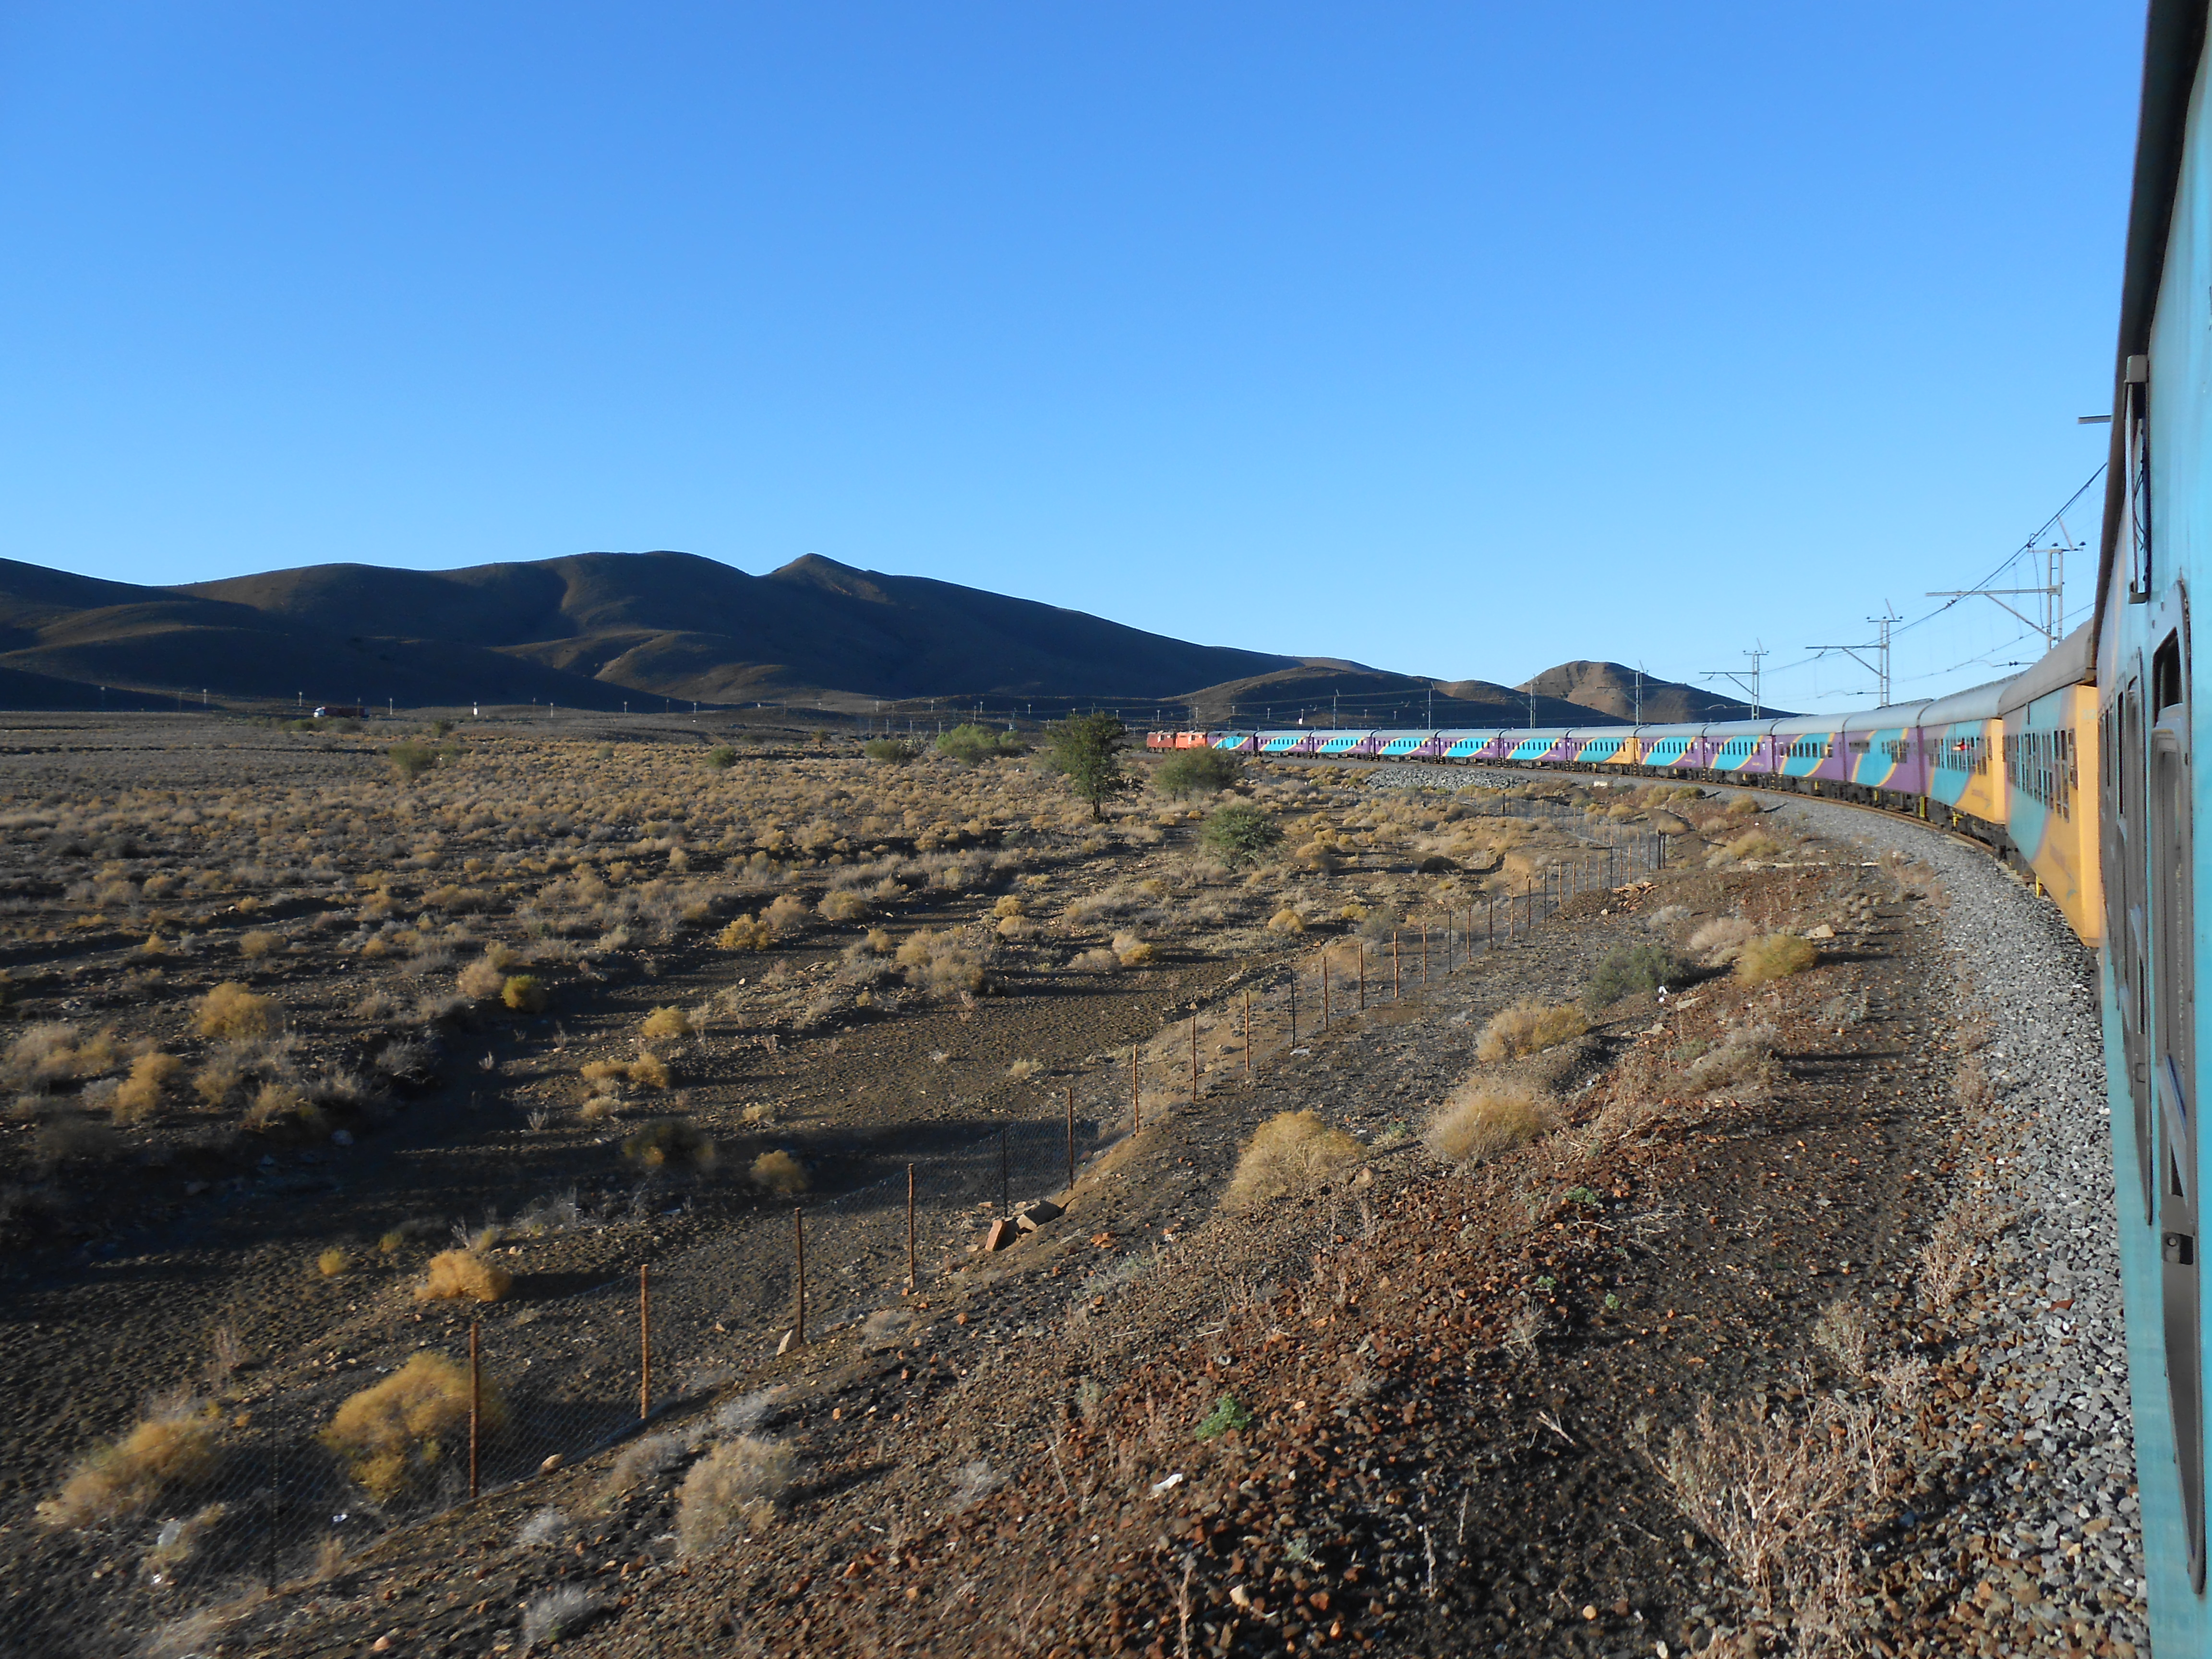
\includegraphics[width=0.4\textwidth]{figures/DSCN0619}\hspace{0.2cm}
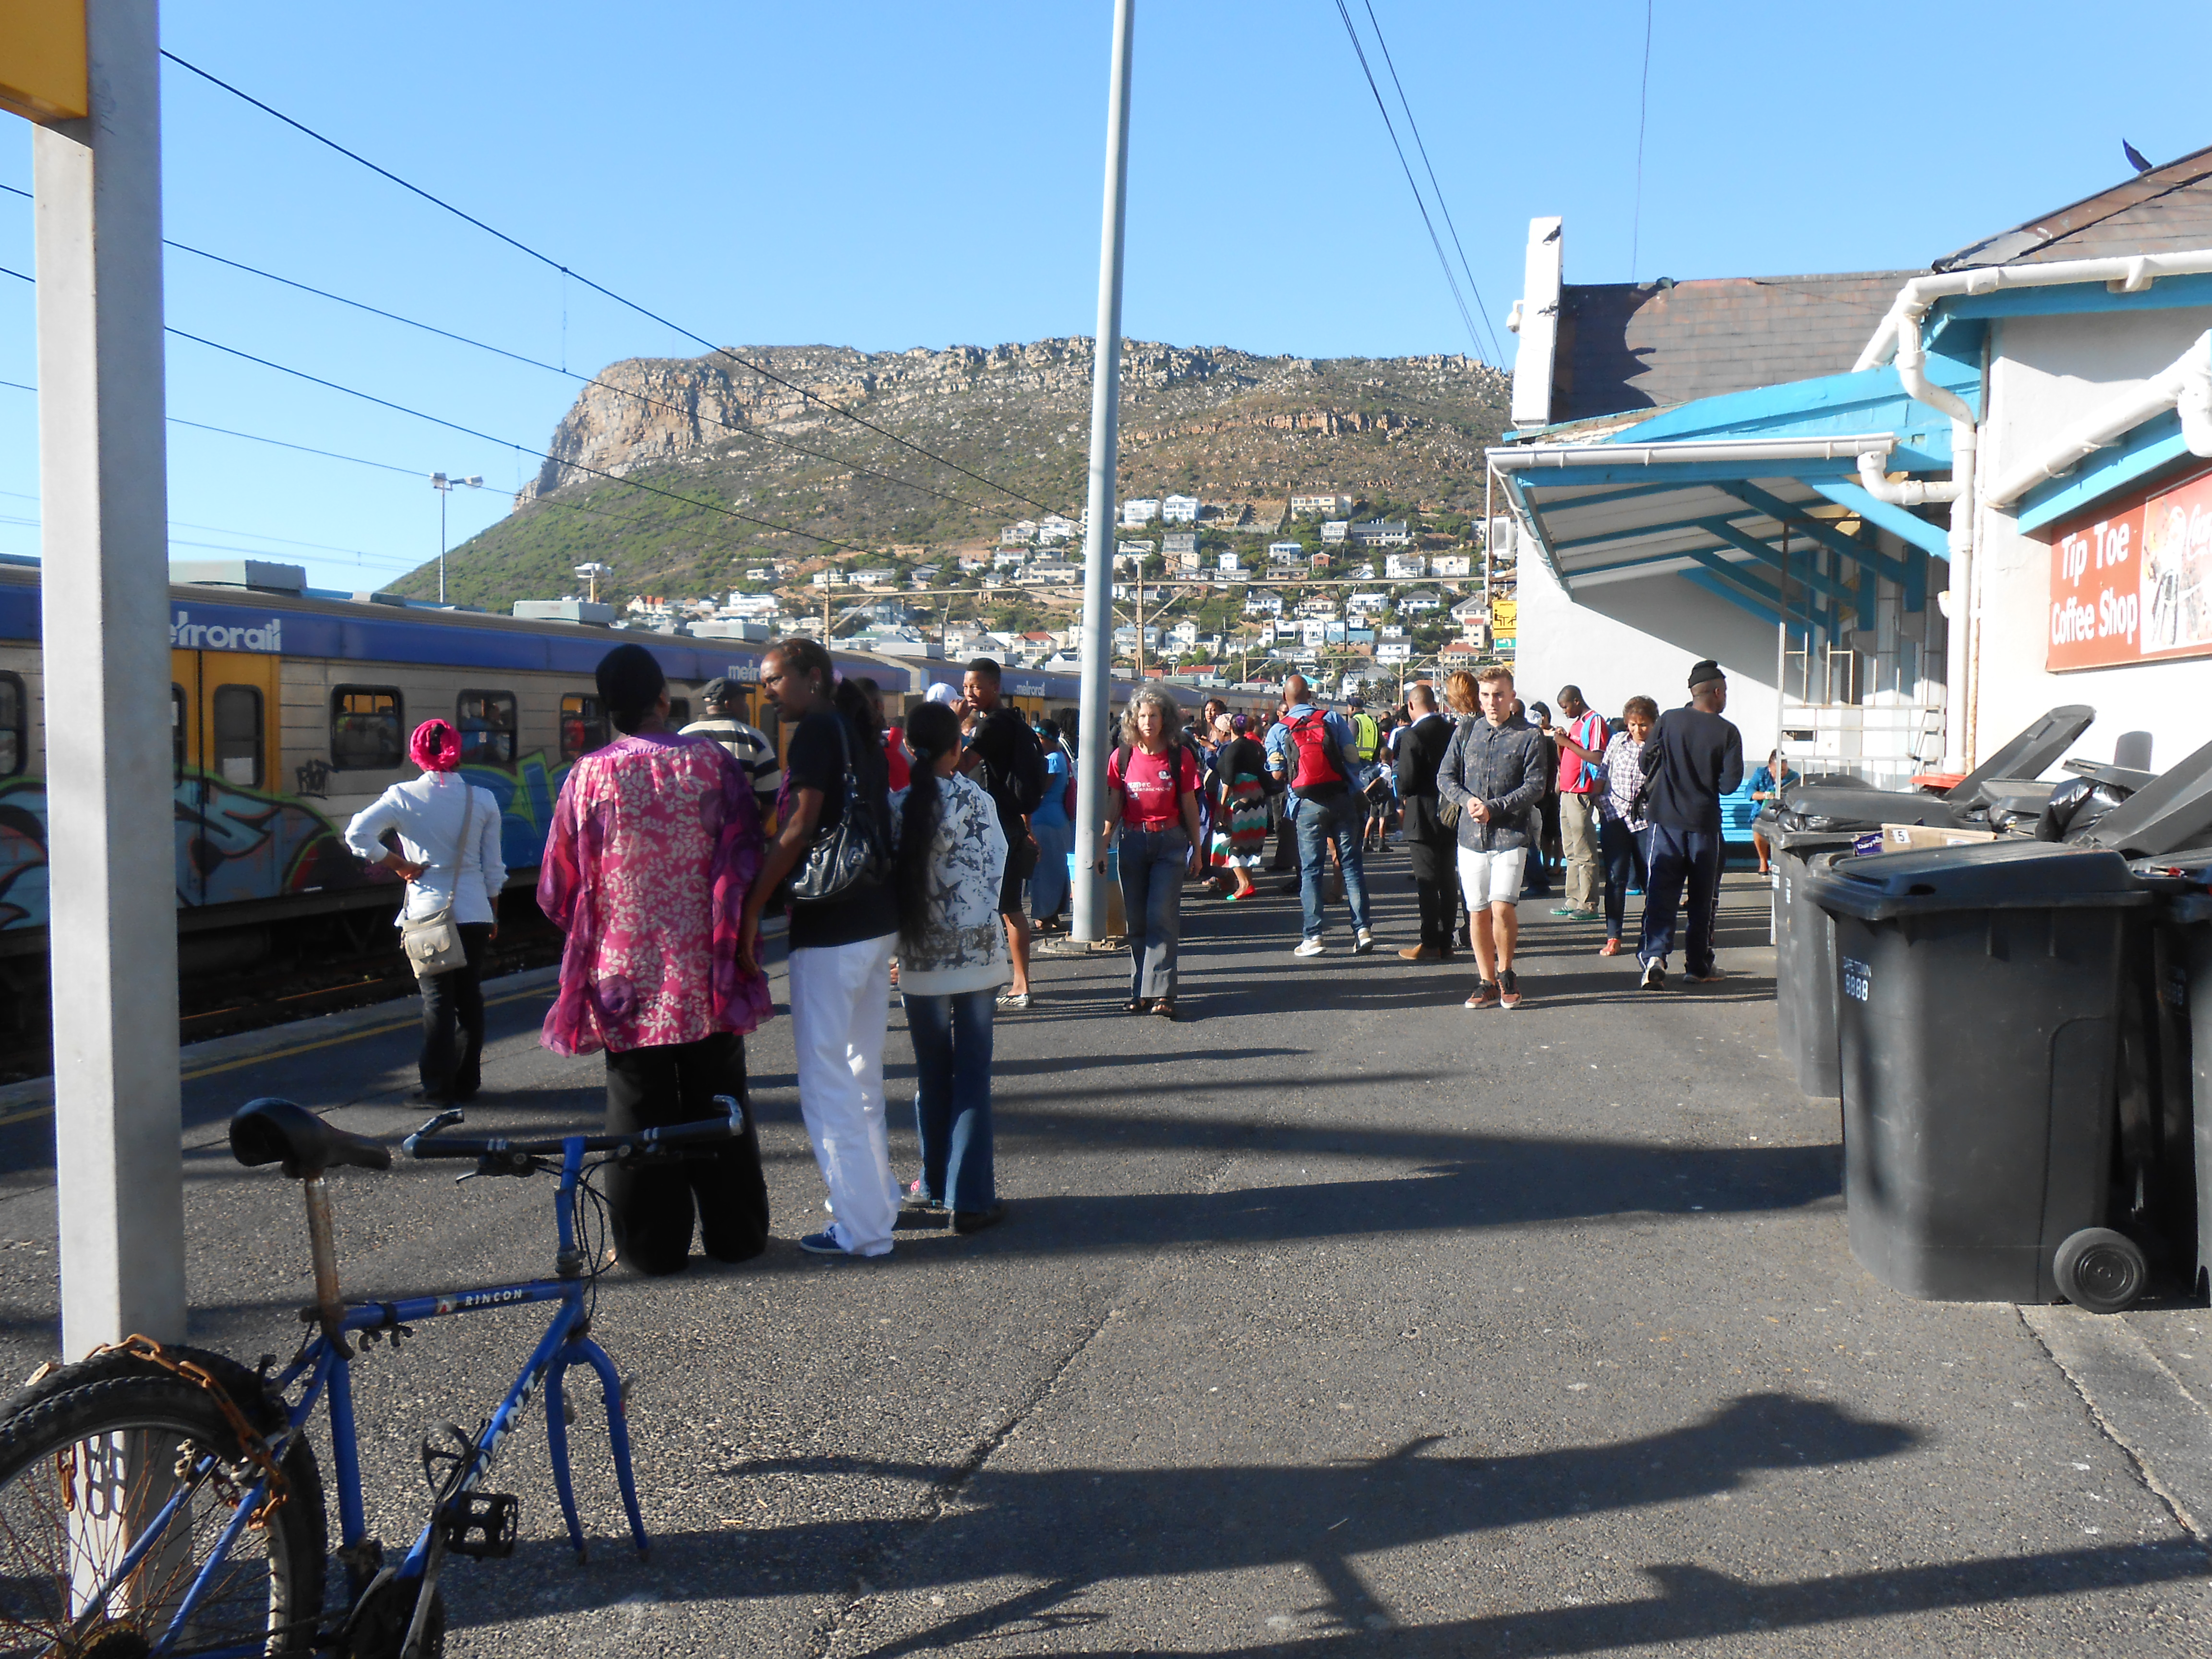
\includegraphics[width=0.4\textwidth]{figures/DSCN1893}\\
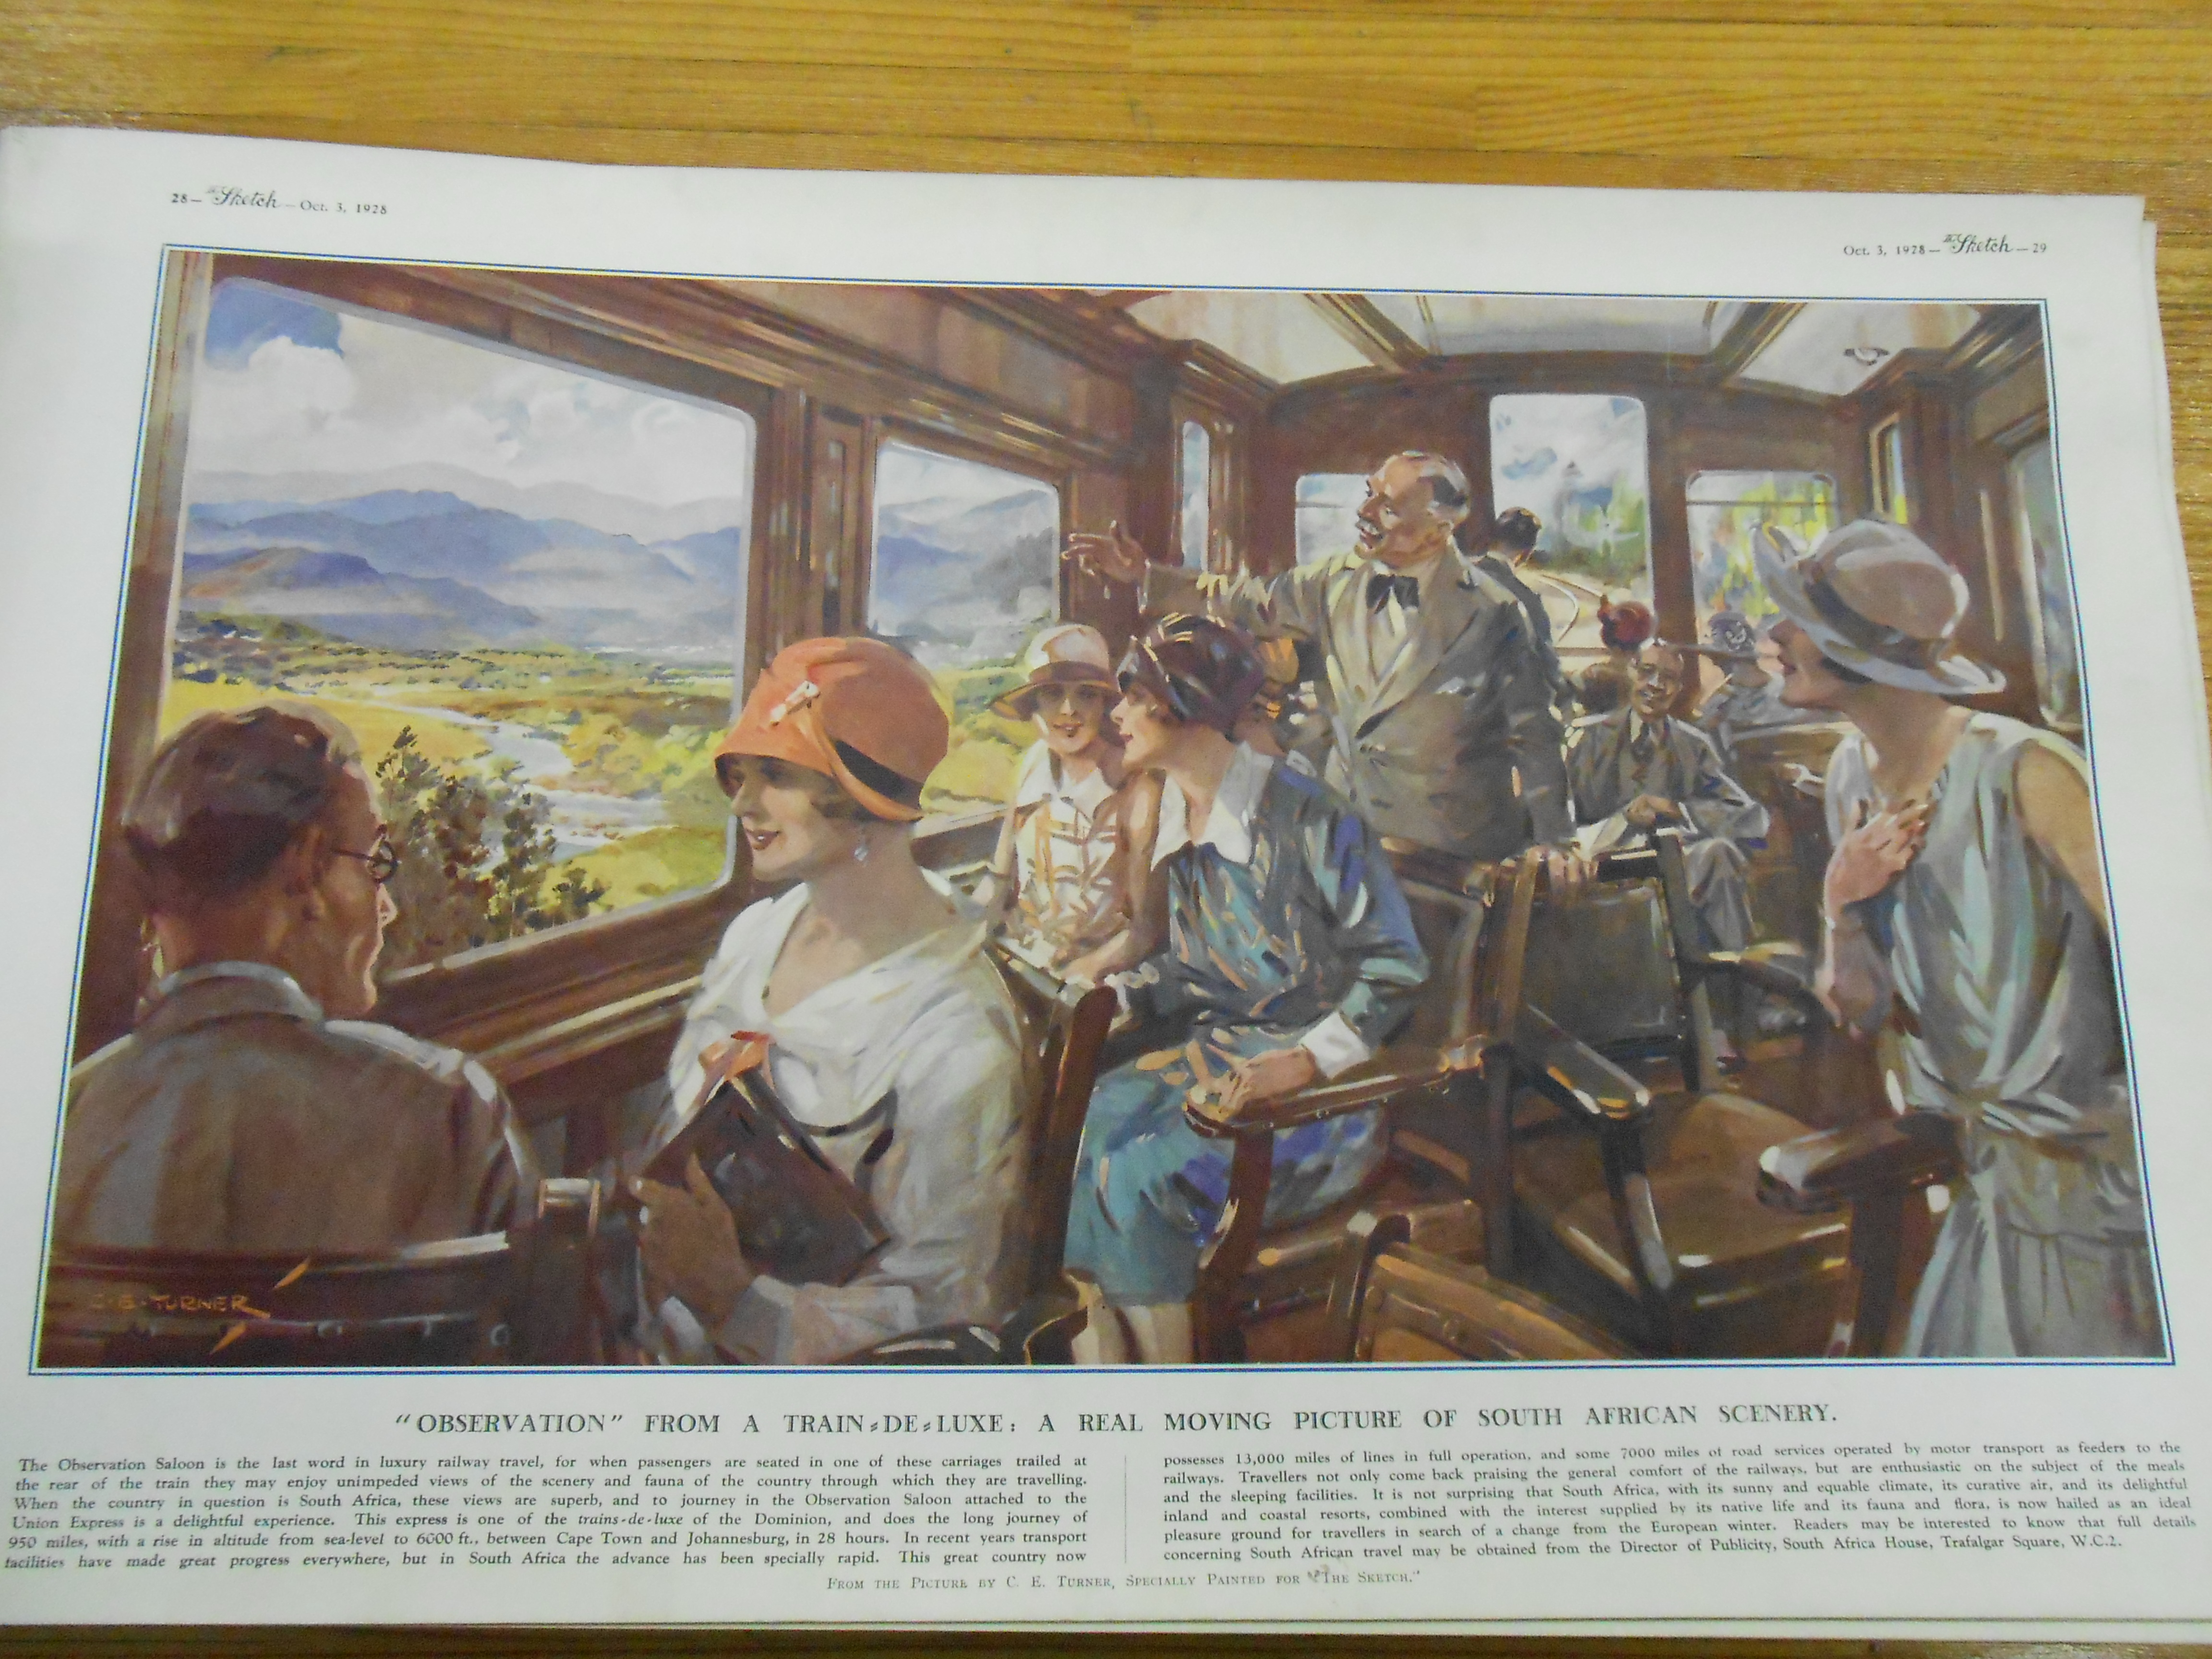
\includegraphics[width=0.4\textwidth]{figures/DSCN0828}\hspace{0.2cm}
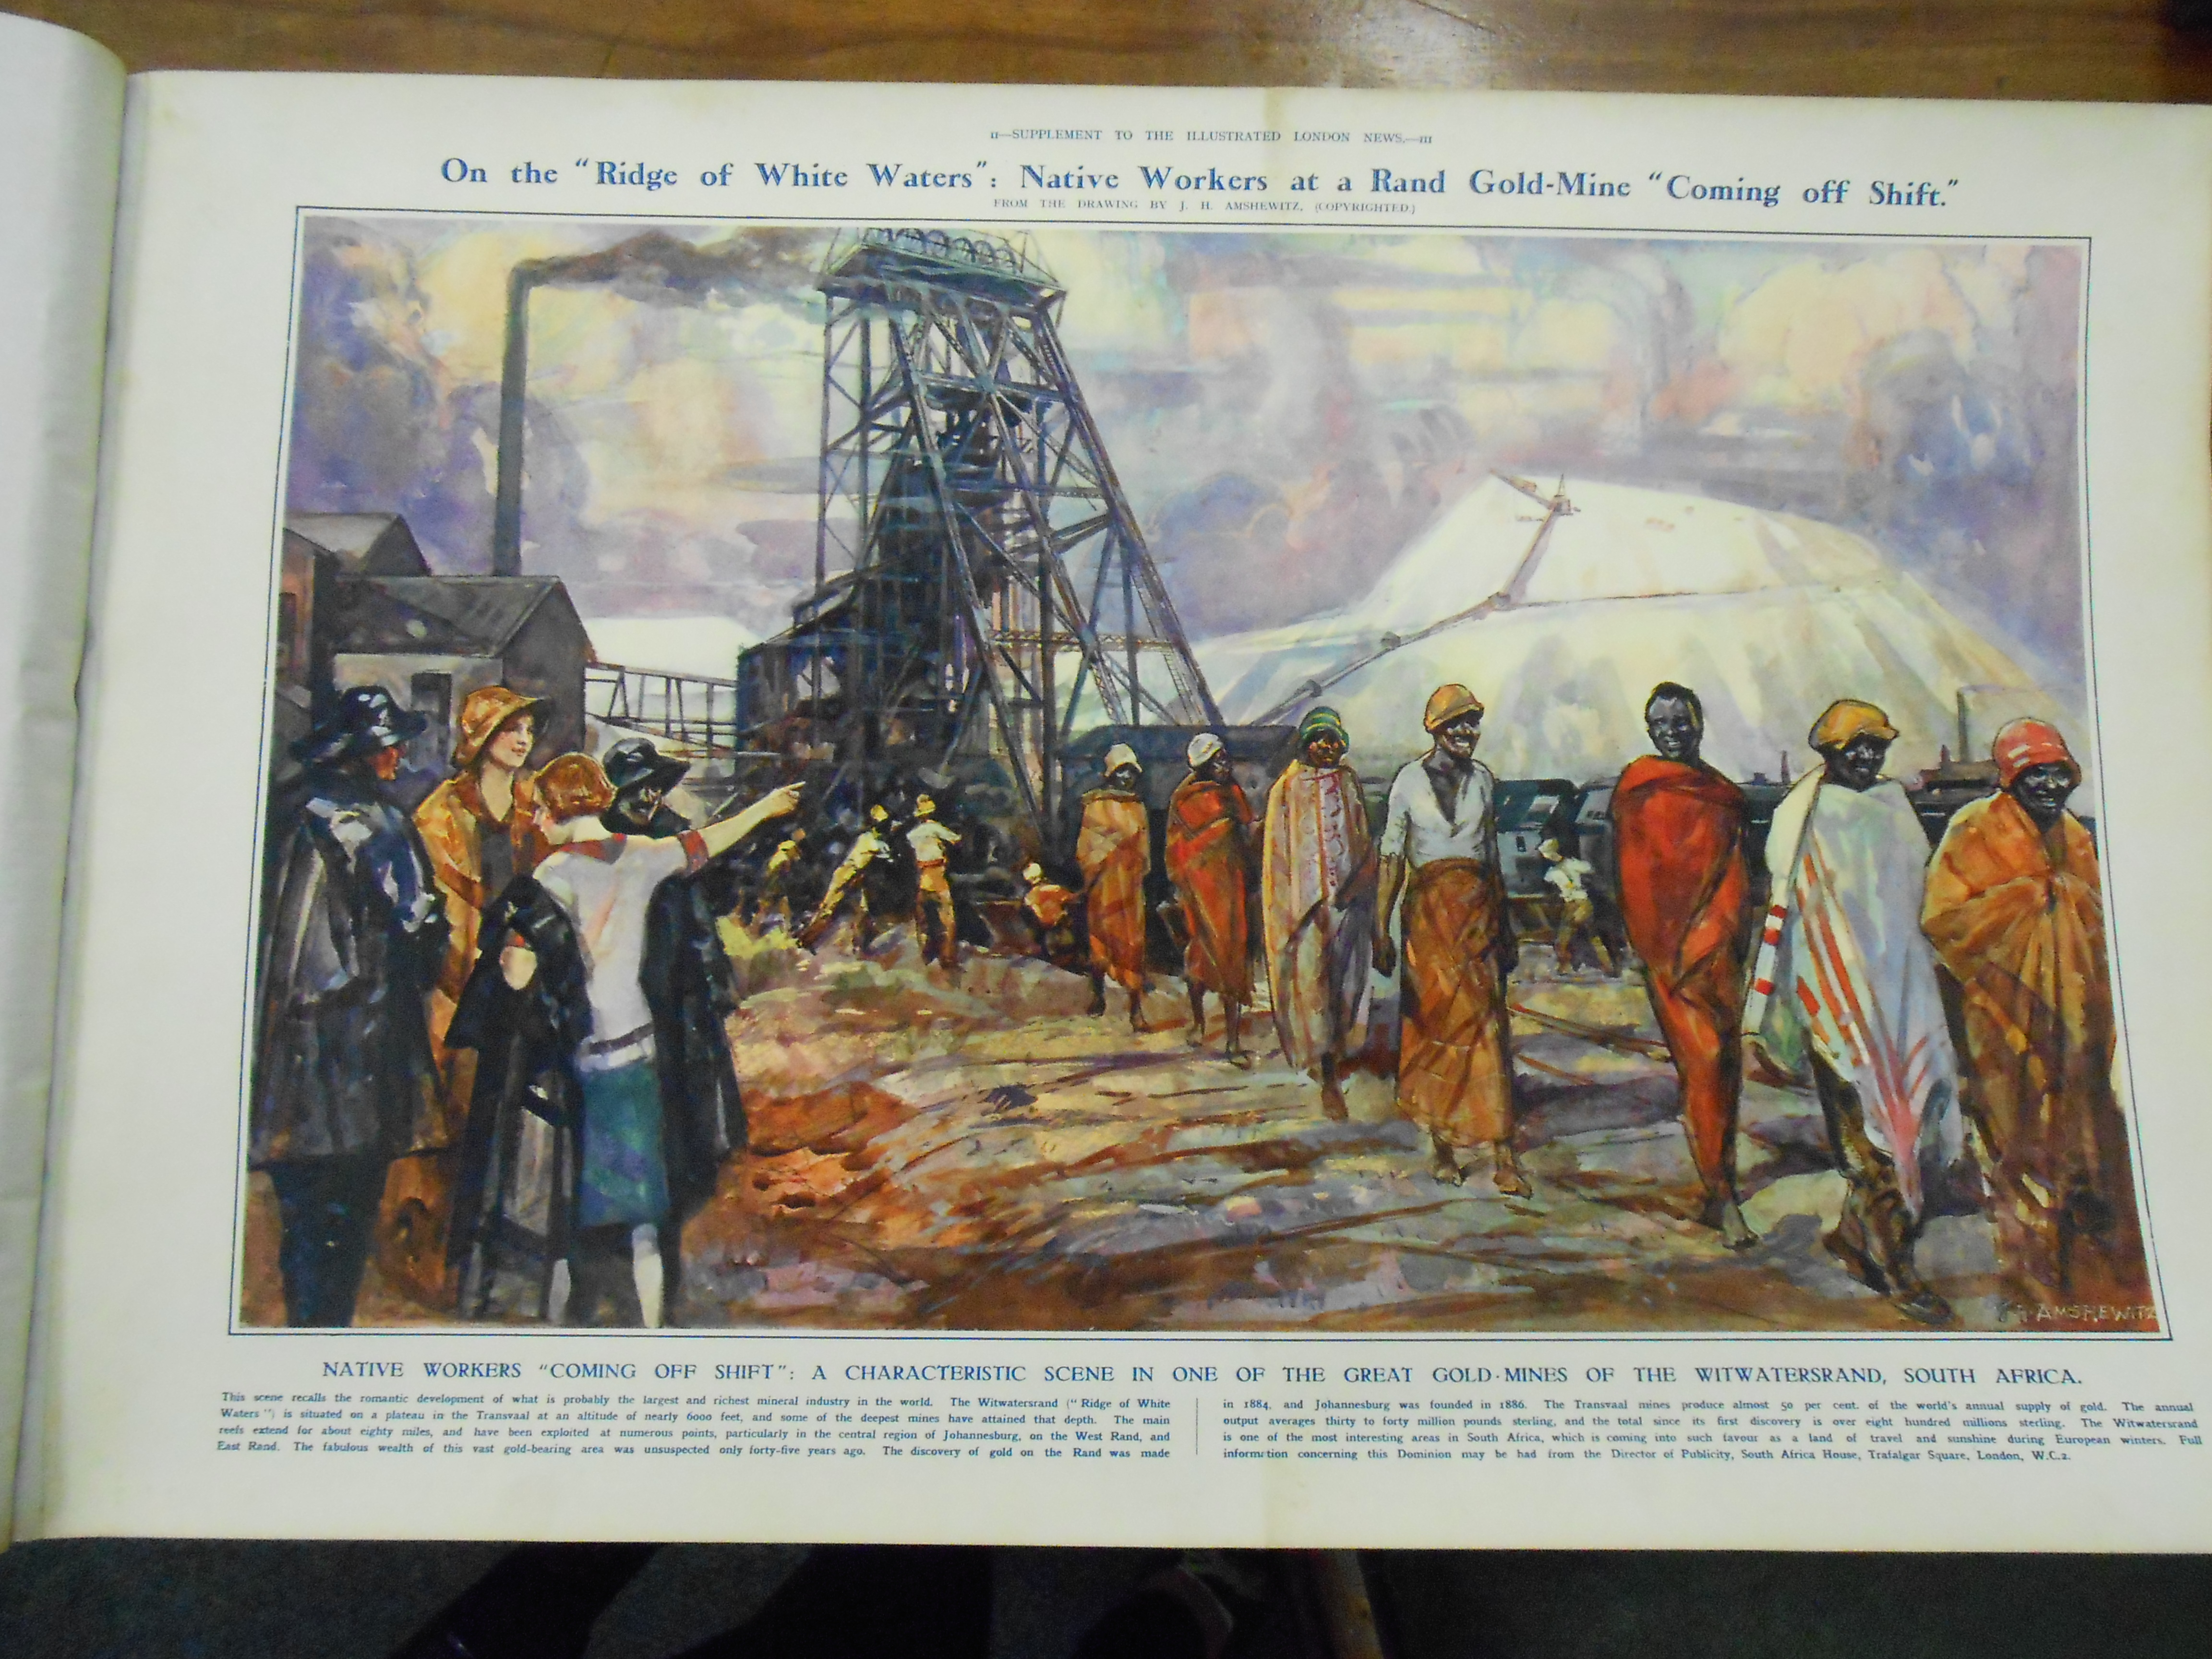
\includegraphics[width=0.4\textwidth]{figures/DSCN0839}


}


%Transportation Networks can be leveraged as a powerful socio-economic control tool, with even more significant outcomes when it percolates to their interaction with territories. The case of South Africa is an accurate illustration, as \cite{baffi:tel-01389347} shows that during apartheid railway network planning was used as a racial segregation tool by shaping strongly constrained mobility and accessibility patterns. We propose to investigate the potential \emph{structural} properties of this historical process, by focusing on dynamical patterns of interactions between the railway network and city growth. More precisely, we try to establish if the segregative planning policies did actually modify the trajectory of the coupled system, what would correspond to deeper and wider impacts.

\sframe{Context}{

\justify

Relations between Network and Territories : complex co-evolutive processes~\cite{bretagnolle:tel-00459720}

\bigskip

$\rightarrow$ \textit{How can these interactions be shaped and leveraged as a socio-economic domination tool ?}

\bigskip

%We use a comprehensive database covering the full South African railway network from 1880 to 2000 with opening and closing dates for each station and link, together with a city database spanning from 1911 to 1991 for which consistent ontologies for urban areas have been ensured. %~(Citation database)\cite{}. %TODO cit. database ?

\textbf{Research Objective : } Using a new population and railway network database on long time span for South Africa~\cite{baffi:tel-01389347}, investigate potential effects of historical events (apartheid segregation laws) on structural properties of the system.


}


\sframe{Interactions between Networks and Territories in South Africa}{

\textit{De-structuring effects of the segregation laws~\cite{baffi:tel-01389347}}

\smallskip

\centering

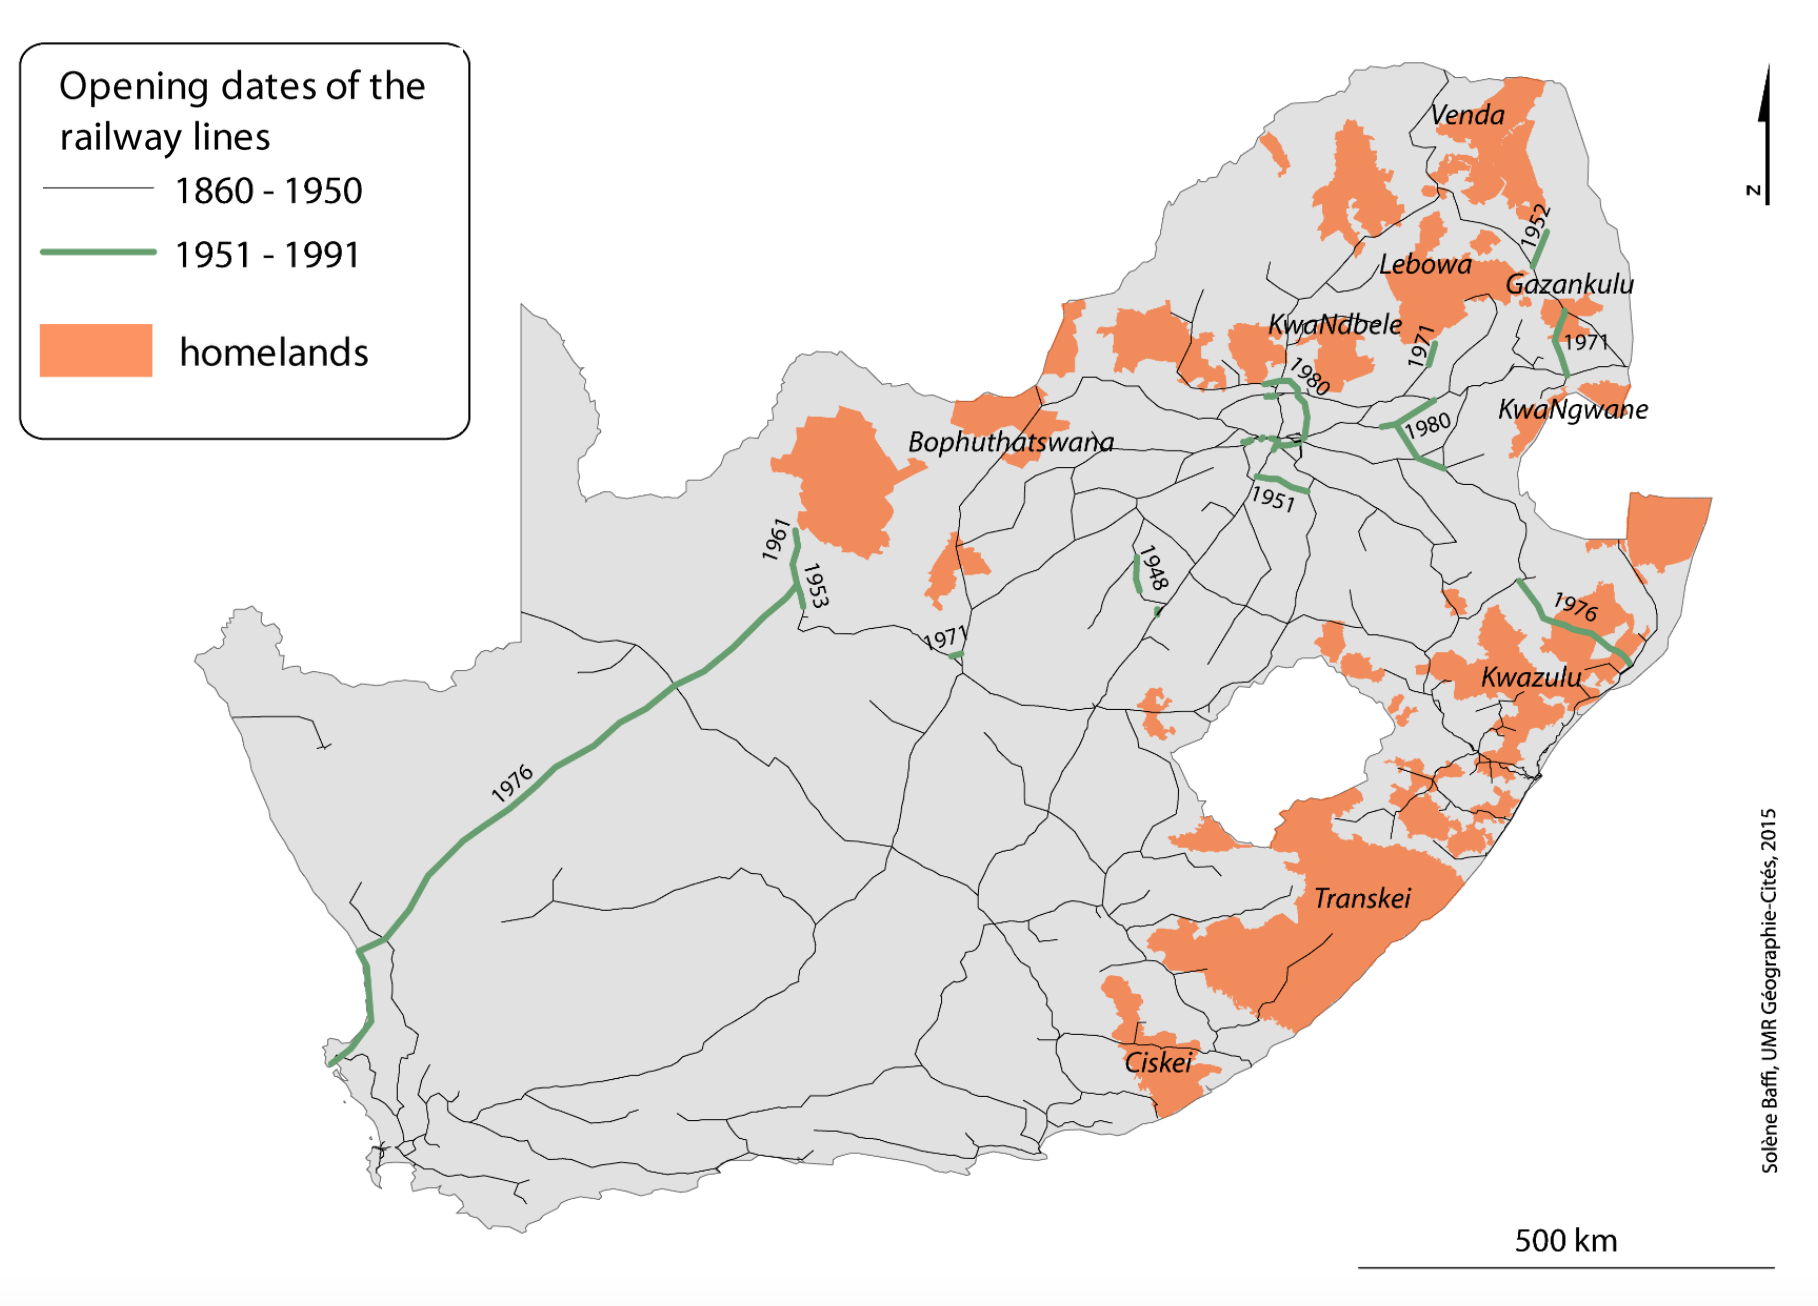
\includegraphics[width=0.8\textwidth]{figures/homelands}

}



%%%%%%%%%%%%%%%%%
\section{Methods and Results}
%%%%%%%%%%%%%%%%%




%First, a dynamical study of network measures seem to confirm the hypothesis: a trend rupture in closeness centrality (defined for a node as the average travel time to other nodes) at a roughly constant network size evolution, at a date corresponding to the beginning of official segregative policies, suggests that the planning process after this date had in the best case no global effect on network performance, and in the worst case had intended negative effects on accessibility with the aim to physically segregate more.

\sframe{Network Analysis}{

\textit{Evolution of Network measures : anomalous trend rupture in centralities}

\medskip

\centering

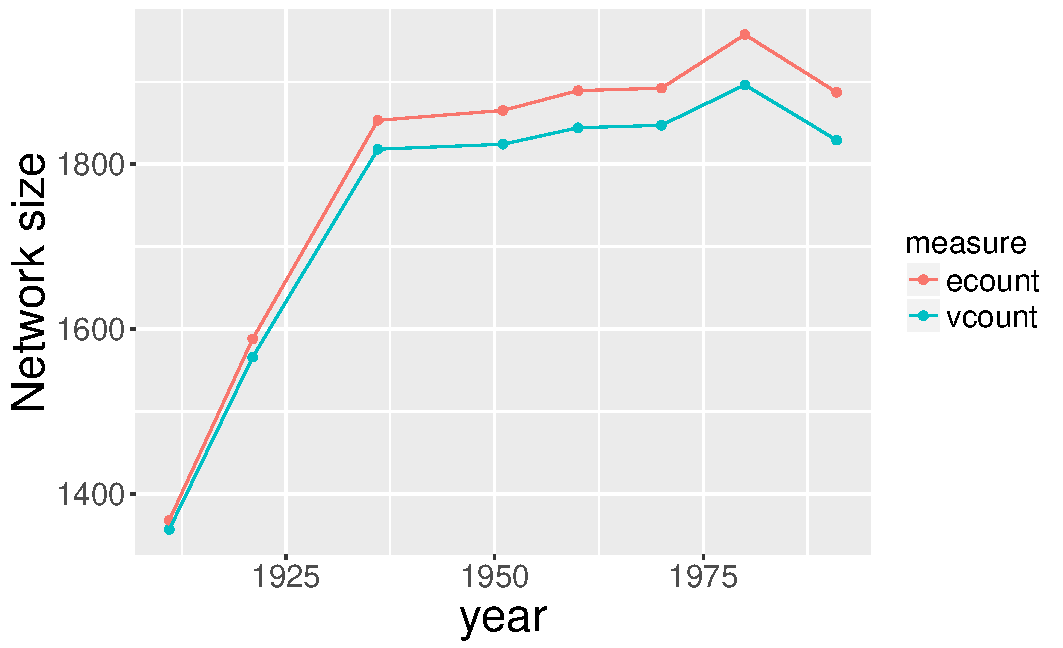
\includegraphics[width=0.4\textwidth]{figures/nw_nwSize}
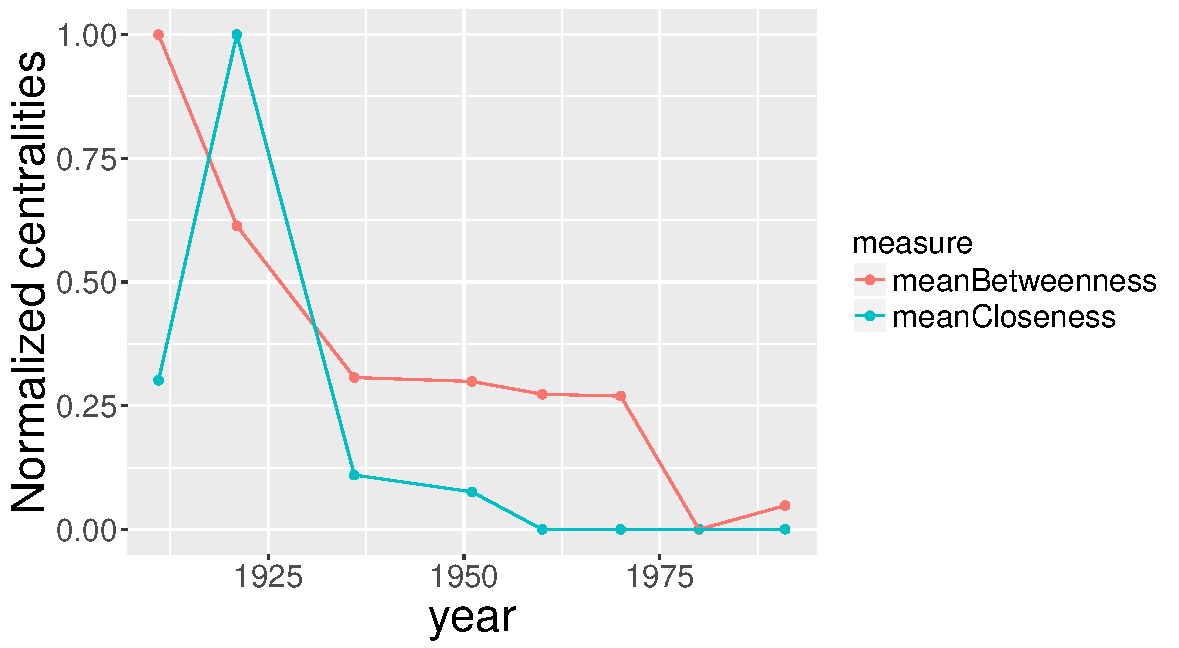
\includegraphics[width=0.45\textwidth]{figures/nw_meanCentralities}\\
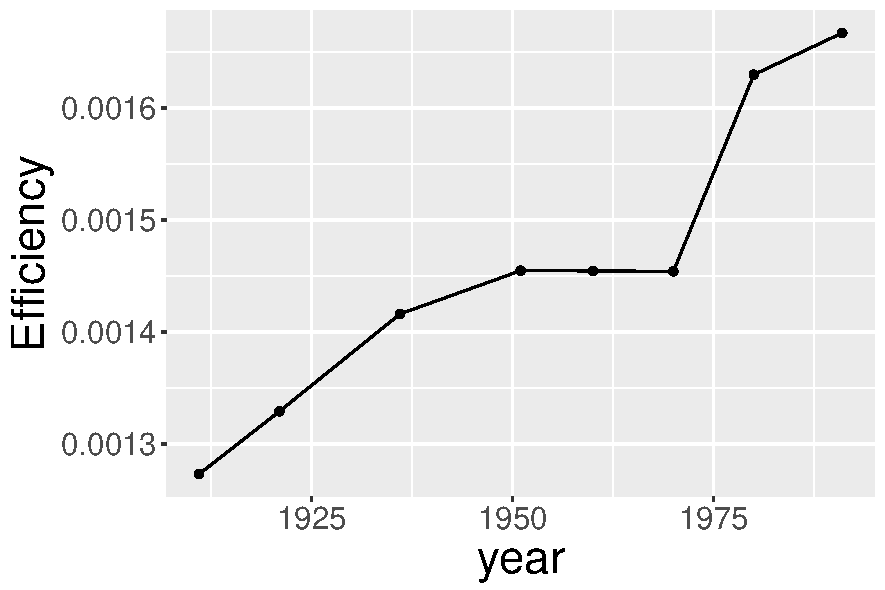
\includegraphics[width=0.4\textwidth]{figures/nw_efficiency}
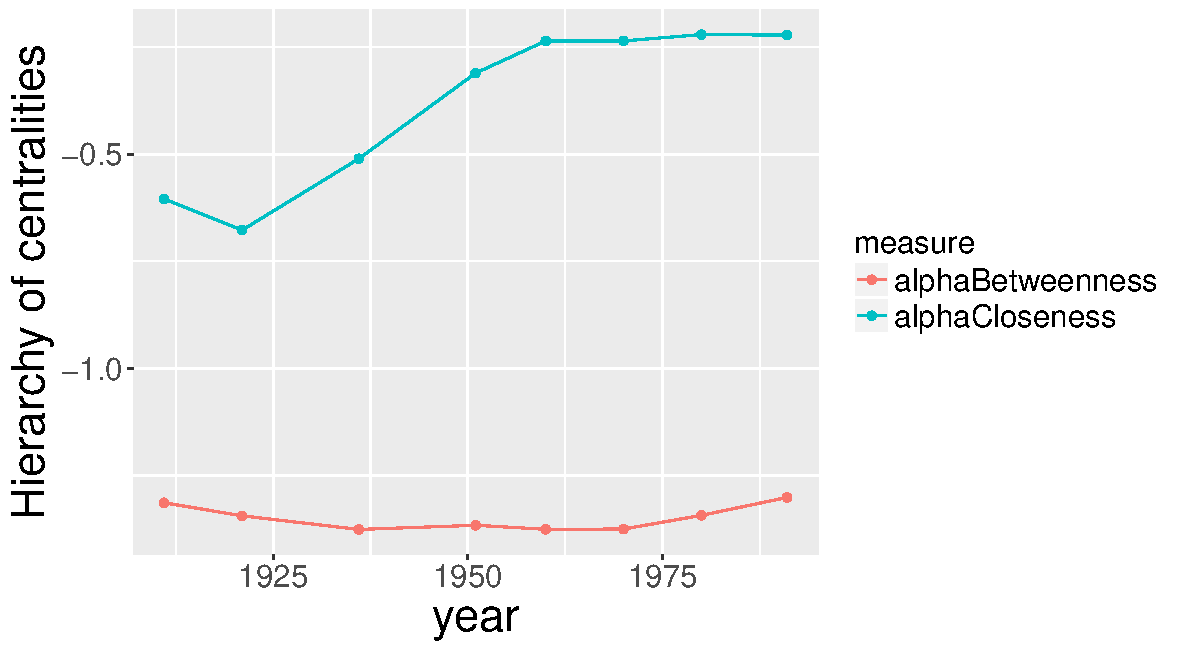
\includegraphics[width=0.45\textwidth]{figures/nw_hierarchies}


}



\sframe{Network Analysis}{

\textit{Connectivity to the railway network : a specific relationship between urban hierarchy and centrality}

\smallskip

\centering

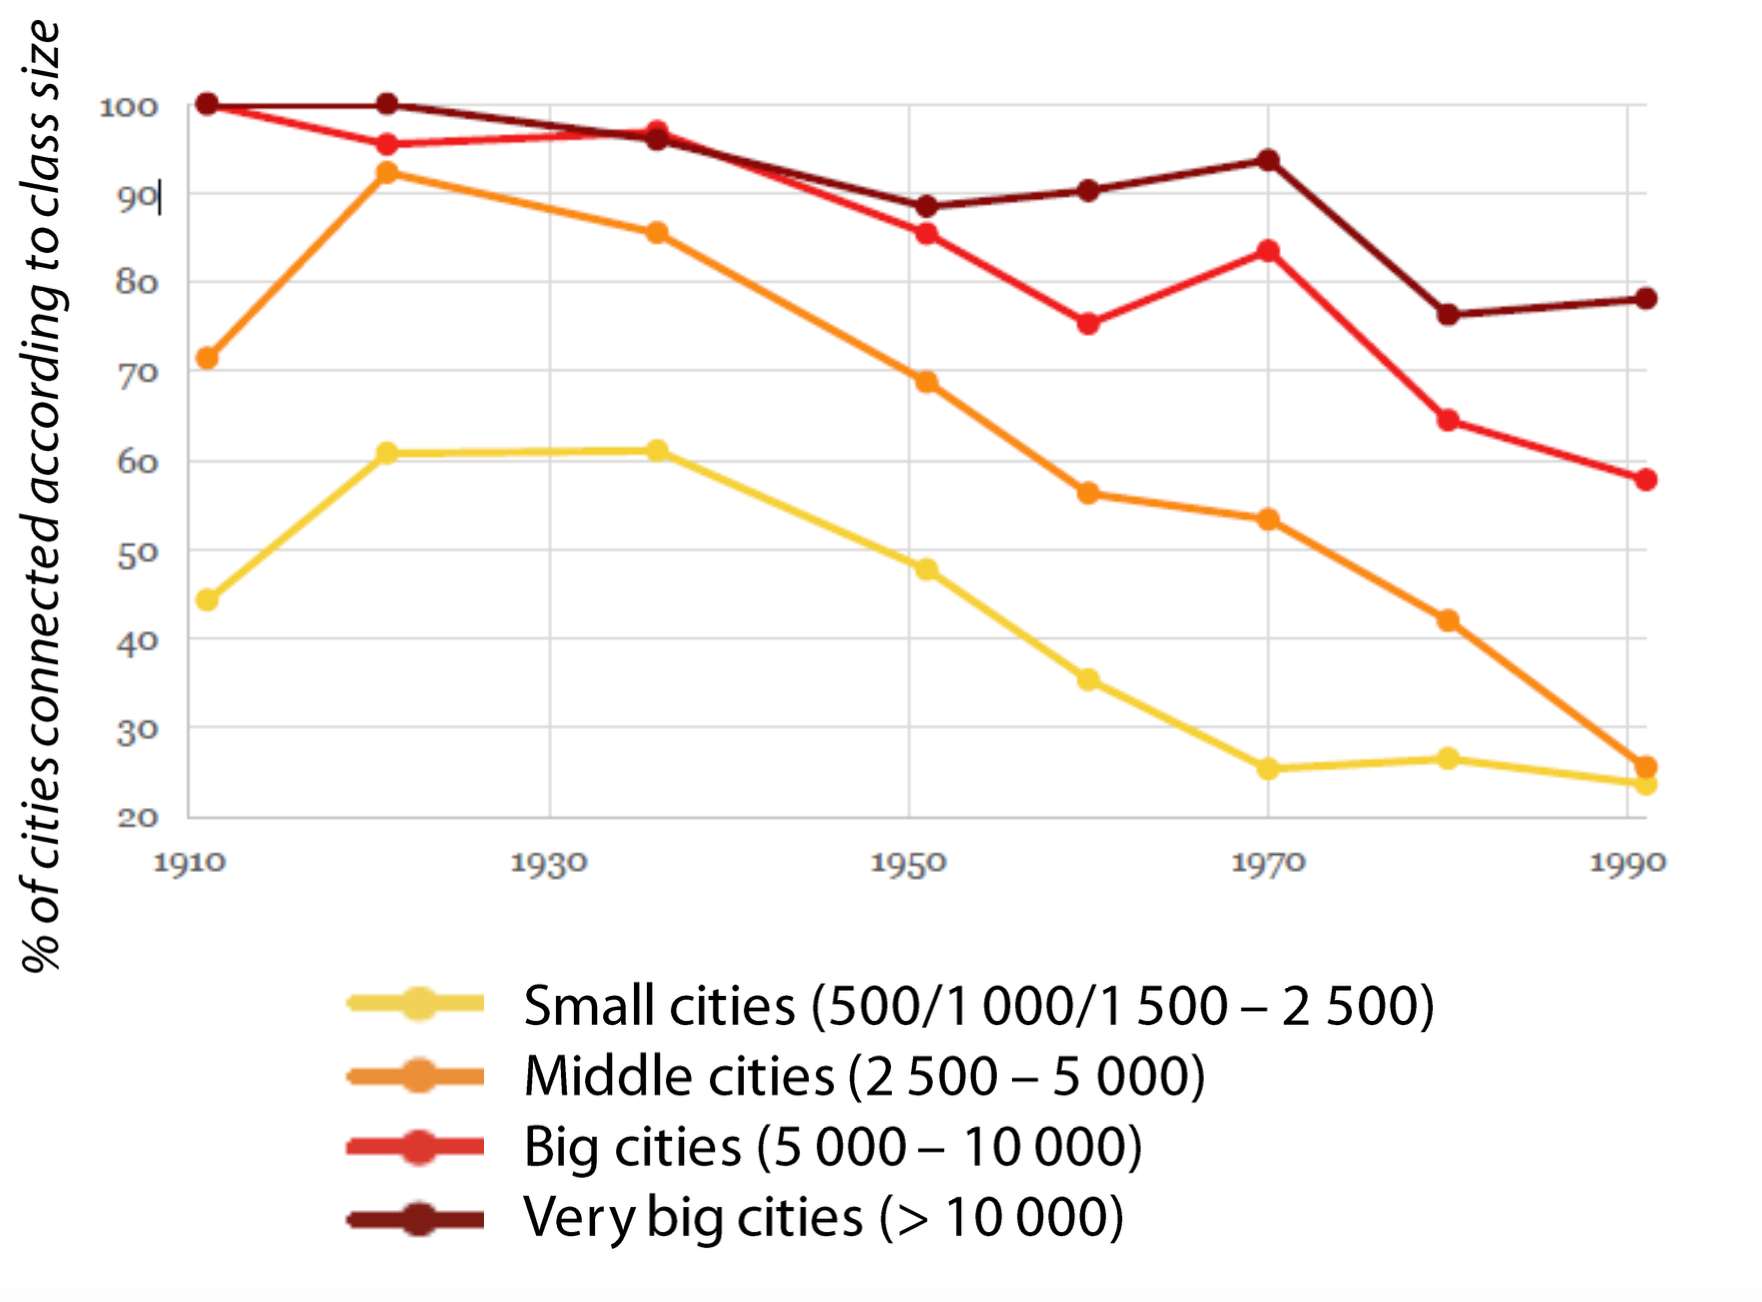
\includegraphics[width=0.8\textwidth]{figures/networkconnection}


}






\sframe{Accessibility Patterns}{

\textit{Distorted co-evolution between cities and the railway network}

\bigskip
\bigskip

\centering

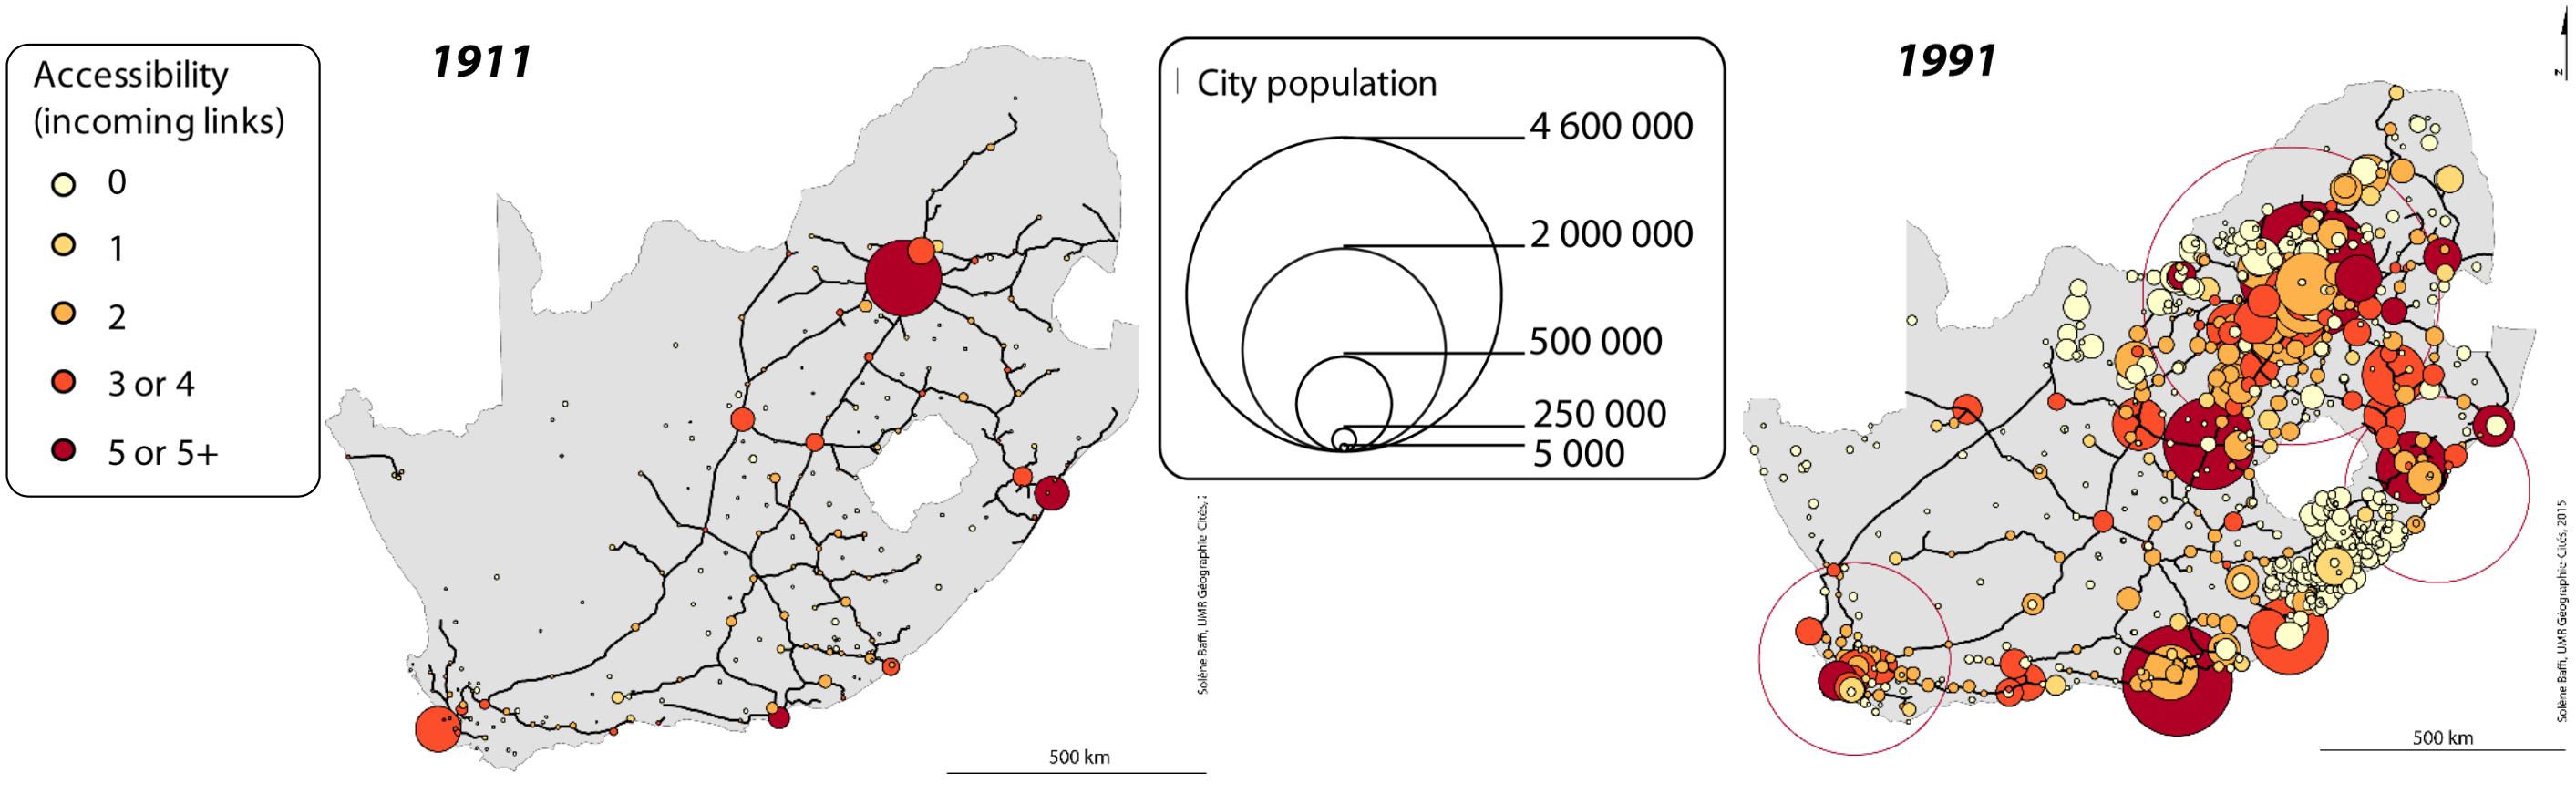
\includegraphics[width=\textwidth]{figures/accessibility-pop.png}


}




%We then turn to dynamical interactions between the railway network and city growth. For that, we study Granger causalities, in the large sense of correlations between lagged variables, estimated between cities growth rates and accessibility differentials due to network growth. %, for all cities and urban areas having a connection to the network.
% We test both travel-time and population weighted accessibilities, for varying values of distance decay parameter. %Lagged correlations are fitted on varying length time windows, to test for potentially varying stationarity scales.
%  We find that results are significant with travel-time accessibility only, autocorrelation dominating with weighted accessibility. A time-window of 30 years appears to be a good compromise between the number of significant correlations ($p<0.1$ for a Fisher test) and the absolute correlation level across all lags and distance decays, what should correspond roughly to the time-stationarity scale of the system.% We observe furthermore a phase transition when distance decay increases, revealing the shift between the spatial scale of urban areas and the scale of the country, what gives local spatial stationarity scale.

\sframe{Spatio-temporal causalities}{

\justify

Use of a generic method to identify causalities in spatio-temporal data~\cite{raimbault2017identification}, in the sense of Granger causalities

\medskip

$\rightarrow$ Estimation of lagged correlations on spatially filtered data, maximising lag if exists (filtering correlations if significant with $p<0.1$ for a Fisher test) gives propagation lag and sense of the causality

\medskip

$\rightarrow$ Spatial aggregation by station ; work with data returns at the first order 

}


\sframe{Stationarity scales}{

\textit{Optimal estimation time window and spatial range for accessibility}


\bigskip

\centering

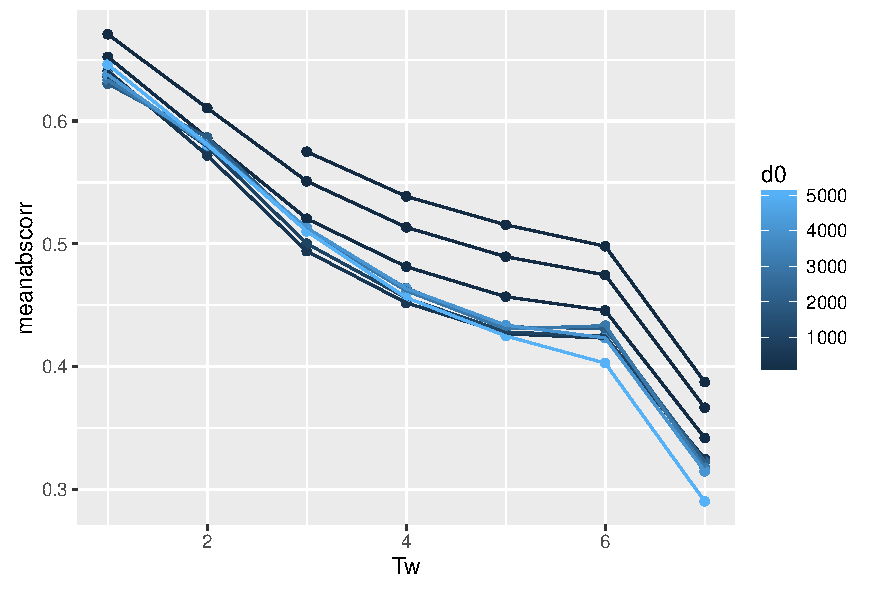
\includegraphics[width=0.5\textwidth]{figures/meanabscorrs}
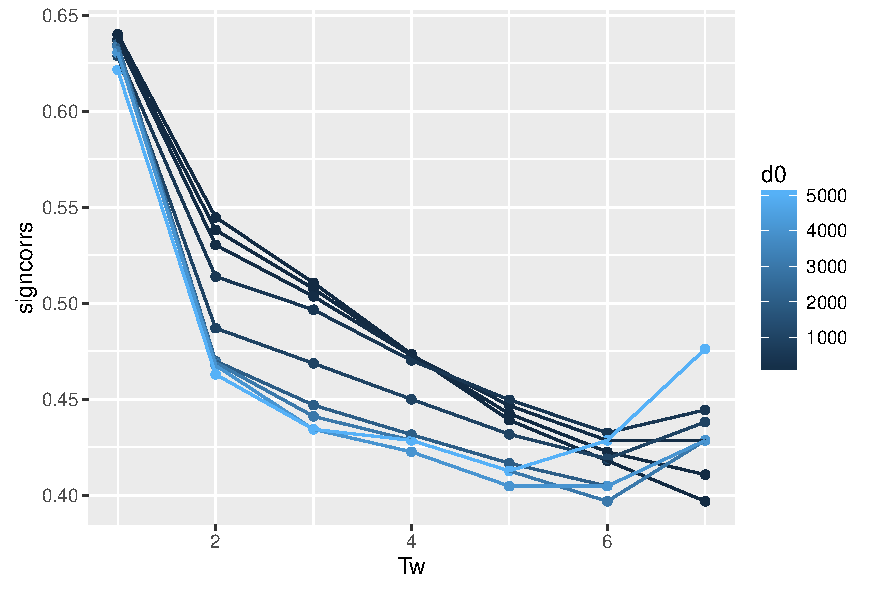
\includegraphics[width=0.5\textwidth]{figures/significantcorrs}

}




%\paragraph{Causality patterns}

%  We obtain therethrough clear causality patterns, namely an inversion of the Granger causality (lagged correlation up to 0.5 for several values of distance decay), from accessibility causing population growth with a lag of 10-20 years before the apartheid (1948), to the opposite after the apartheid (lag 20 years). We interpret these as \emph{Structural segregation}, i.e. a significant impact of planning policies on dynamics of interactions between networks and territories. Indeed, the first regime corresponds to direct effect of transportation on migrations in a free context in opposition to the second one. Further work should consist in similar study with more precise socio-economic variables, for example quantifying directly segregation patterns.




\sframe{Causality Patterns}{

\textit{Clear inversion of the sense of Granger causality suggests a structural segregation effect of the apartheid laws}

\bigskip

\centering

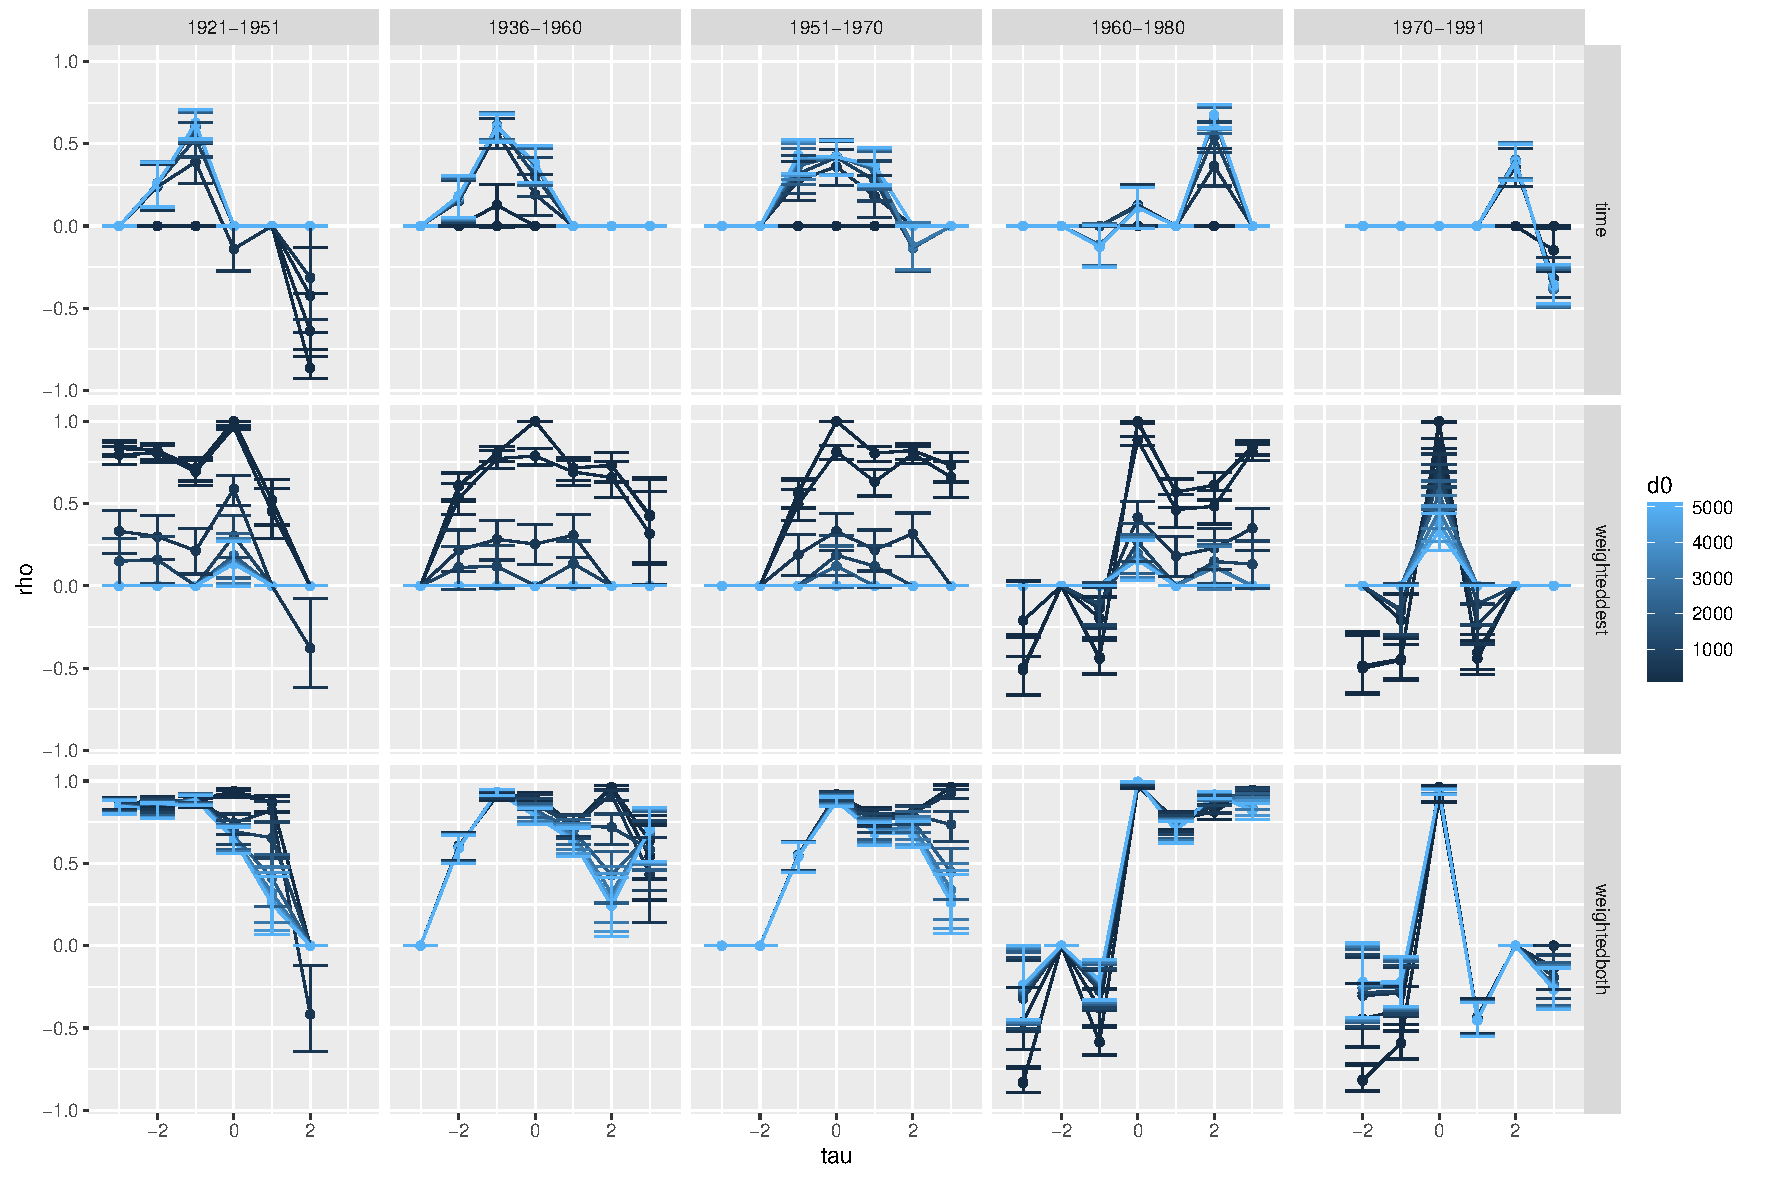
\includegraphics[width=0.82\textwidth]{figures/laggedCorrs_Tw3}

}


%%%%%%%%%%%%%%%%%
\section{Discussion}
%%%%%%%%%%%%%%%%%





\sframe{Discussion}{

\justify

\textbf{Implications}

$\rightarrow$ Existence of a \textit{Structural Segregation}, in the sense of an impact of policies on second-order dynamics of the system

\medskip

$\rightarrow$ Co-evolutive processes becoming de-structuring, the rail being used as a tool of power

\bigskip

\textbf{Developments}

$\rightarrow$ Relations with more precise socio-economic variables, direct segregation patterns, housing market, power relations and socio-economic activities~\cite{migozzi2010rugby}

\medskip

$\rightarrow$ Method of statistical instrumentation using beginning/end of apartheid as an exogenous independent shock~\cite{angrist1996identification}

}




\sframe{Conclusion}{

\justify

$\rightarrow$ Converging evidences and complementary approaches to unveil particular cases of co-evolutive dynamics

\medskip

$\rightarrow$ Crucial aspect of both empirical and theoretical domains, and of concrete fieldwork surveys to fully interpret numerical analyses

\bigskip
\bigskip
\bigskip


\footnotesize{ - Code et data available at\\ \texttt{https://github.com/JusteRaimbault/CityNetwork/tree/master/Models/}
\\\texttt{SpatioTempCausality/SudAfrica}
}

}






\sframe{Reserve slides}{

\centering

\Large

\textbf{Reserve Slides}

}


\sframe{Apartheid policy}{

\begin{itemize}
%À l’origine de la politique d’apartheid, deux objectifs déterminent l’ensemble des mesures politiques qui sont instaurées pendant la durée du régime : la promotion d’un développement séparé, et le maintien de la prospérité économique des Afrikaners. Ce second objectif implique une dépendance forte à la main d’œuvre très bon marché que constitue la population africaine, majoritaire dans le pays. Cet impératif justifie, d’après D. Posel (2011, p. 322), que la politique d’apartheid n’ait jamais eu pour but direct l’extermination, à l’instar d’autres politiques racistes comme le nazisme. Outre la déshumanisation que subissent les populations non-blanches pendant les années d’apartheid, celles-ci sont alors considérées comme une ressource économique nécessaire au bon fonctionnement du système économique d’apartheid, une ressource indispensable bien qu’indésirable.
\item Deshumanized colored populations and exploitation as a crucial economic ressource, to sustain economic prosperity of afrikaners population
%La mise en place d’une politique de développement séparé nécessite alors une mise à distance négociée : la séparation spatiale entre les différents groupes de population ne doit pas entraver l’accès des populations ségrégées aux zones d’emploi. C’est dans cette optique que sont instaurés des espaces ségrégés à l’échelle interurbaine et intra-urbaine, résultant de l’imposition du « grand apartheid ». Celui-ci instaure la division spatiale à l’échelle de la ville (par la création de townships) et du pays. À l’échelle du pays, la séparation concerne essentiellement la population africaine : les autres groupes raciaux, les Coloureds et les Indiens se concentrent très majoritairement dans les centres urbains. À partir des années 1970 les anciennes réserves africaines héritées de la période coloniale se transforment en bantoustans qui correspondent chacun à une ethnie différente. Pour ce faire, le gouvernement décompose le groupe de population africaine en neuf « familles linguistiques » (Zulu, Xhosa, Tswana, Sotho du Nord et Sotho du Sud, Swazi, Ndebele, Venda et Shangaan) et attribue à chacun un territoire distinct. Six de ces bantoustans appartiennent à la catégorie de territoires autonomes (Gazankulu, Lebowa, Qwaqwa, Kanguane, Venda, KwaNdebele) et quatre sont progressivement déclarés indépendants (le Transkei en 1972, le Bophuthatswana en 1973, le Venda en 1979 et le Ciskei1 en 1981). Ces territoires, qu’ils soient autonomes ou indépendants, se gèrent eux-mêmes et reçoivent une allocation gouvernementale. 
\item Planned spatial division at different scales : specific autonomous regions called bantoustans
%Chaque individu africain ne bénéficiant pas d’un contrat de travail auprès d’un employeur blanc est contraint de résider dans l’un des dix bantoustans qui relève de son ethnie (Gervais-Lambony, 1997, p. 50). Les industries sont incitées à venir s’installer aux frontières de ces territoires par des mesures économiques attractives, mais certains des bantoustans, situés parfois à des centaines de kilomètres des zones d’emplois, requièrent la mise en place de réseaux de bus et de trains pour assurer les mobilités quotidiennes ou hebdomadaires des travailleurs. La nouvelle géographie nationale implique donc la création de lignes ferroviaires à même d’entretenir les mobilités d’une population indispensable au fonctionnement économique du système d’apartheid mais volontairement tenue à distance. L’ouverture des lignes ferroviaires pendant la période d’apartheid répond ainsi à cette logique
\item Residential constraints depending on employment status and ethnic origin
%Des lignes relient directement certains bantoustans à des centres urbains, comme la connexion établie entre le Bophuthatswana et le Gauteng. Dans d’autres cas, des lignes sont construites dans l’objectif de raccorder le bantoustan à l’ensemble du réseau, notamment au Kwazulu, au Lebowa ou au Gazankulu. L’accessibilité permise par le réseau ferroviaire autorise alors la main d’œuvre à atteindre plus rapidement les centres miniers où elle est employée.
\item Railway network designed to optimize commuting for mines workers
%L’économie d’apartheid repose alors sur les migrations d’une partie importante de la main d’œuvre africaine. Les migrations de travail de la population africaine préexistent à l’apartheid, toutefois elles évoluent dans leurs formes et leur intensité durant cette période. Dans le cas des individus déplacés vers les bantoustans et employés en Afrique du Sud, les migrations de travail impliquent désormais parfois le franchissement d’une frontière internationale, étant donné que l’État d’apartheid reconnaît certains de ces territoires comme des États indépendants ou autonomes. Les effectifs des migrants augmentent au cours de la période, en particulier après 1968. D’après G. Pirie (1992, p. 173), en 1984, le nombre de navettes quotidiennes depuis les bantoustans s’élève à 2,1 millions, et concerne une proportion importante de la population de ces territoires. Après cette date, les Africains ne sont plus autorisés qu’à louer des maisons dans les townships des villes « blanches » lorsqu’ils ont accès à celles-ci, et sont encouragés à construire une résidence dans le périmètre de leur bantoustan. Le déplacement forcé de ces populations vers des territoires distants a des répercussions directes en matière de transport : les navettes quotidiennes de la main d’œuvre s’allongent, tandis que la majorité de ces employés ne peut plus assumer le coût de déplacement induit. Des subventions sont alors instituées par le gouvernement pour maintenir les migrations : une partie des coûts est prise en charge par l’État, l’autre par l’employeur (Lemon, in Smith, 1982). 
\item High level of induced migrations : up to 2.1 millions daily commutes in 1984
\end{itemize}

}

\sframe{Defining co-evolution}{

\justify

No clear definition of co-evolution in the literature : \cite{bretagnolle:tel-00459720} distinguishes ``reciprocal adaptation'' where a sense of causality can clearly be identified, from co-evolutive regimes 

\bigskip

\cite{raimbault2017identification} identifies multiple causality regimes in a simple strongly coupled growth model $\rightarrow$ to be put in perspective with a theoretical definition of co-evolution based on the conjunction of Morphogenesis and the Evolutive Urban Theory, summarised by~\cite{raimbault2017co}


}

\sframe{Database}{

\begin{itemize}
	\item Consistent ontologies for metropolitan areas
	\item Precisely geocoded stations and rail network (with dates of opening and closing) from historical maps and secondary sources
	\item Growth rates and correlations computed on connected cities
\end{itemize}

}


\sframe{Accessibility}{

 $P_i$ populations, $d_{ij}$ network distance matrix, accessibility is given for $i$ by
  \[Z_i = w_i \sum_j w_j \exp \left(- d_{ij} / d_0 \right)\]
  with $d_0$ decay parameters and weights $w_i$ are $1/N$ or $P_i / \sum_j P_j$ depending on weighting scheme.
  
}


%%%%%%%%%%%%%%%%%%%%%
\begin{frame}[allowframebreaks]
\frametitle{References}
\bibliographystyle{apalike}
\bibliography{/Users/juste/ComplexSystems/CityNetwork/Biblio/Bibtex/CityNetwork,biblio}
\end{frame}
%%%%%%%%%%%%%%%%%%%%%%%%%%%%









\end{document}







